\chapter{Introduction}
\label{chap:introduction}

In the last 100 years, power consumption has increased rapidly, and power production is likewise becoming more important \cite{powerconsumption}. Such an increase introduces a great challenge since green energy production has difficulty keeping up with the rising demand. In the current state, we are involuntarily using an equally increasing amount of fossil fuels, which solves the energy problem but introduces several environmental consequences. With more than 70 countries committing to "net zero" energy production in the near future, the importance should not be overlooked. According to the International Energy Agency \cite{powerconsumptiongraph}, this goal is reachable in 2050 on the condition that power production is drastically alternated. As seen in figure \ref{fig:powerdistribution}, the required energy source distribution needs to change substantially, with especially solar and wind energy becoming more prevalent.

\begin{figure}[H]
    \centering
    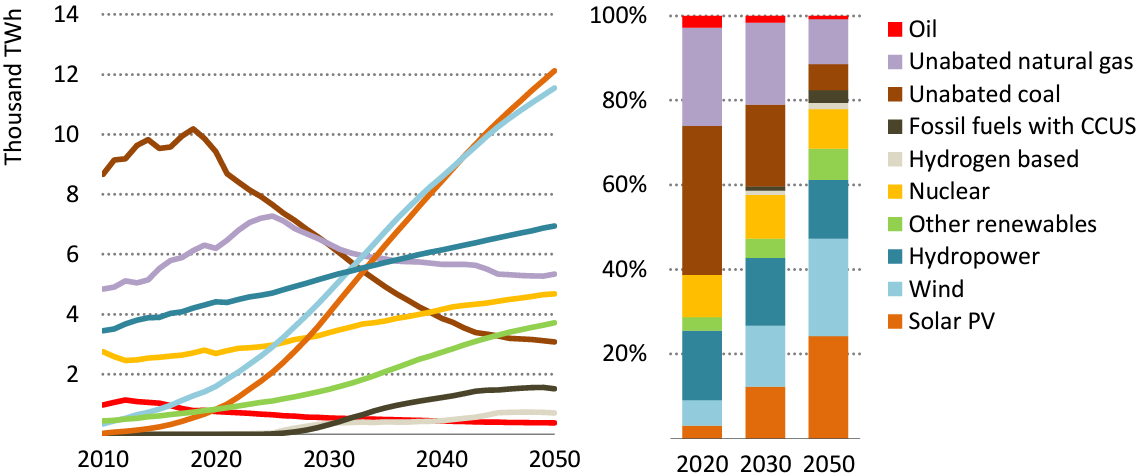
\includegraphics[scale=0.45]{Illustrations/Distribution of power production.png}
    \caption{Distribution of power production. \cite{powerconsumptiongraph}}
    \label{fig:powerdistribution}
\end{figure}

Because of this need to increase energy production by turbines, it is now more relevant than ever to optimise existing as well as new farms for them to reach their maximum efficiency. One of the many challenges when planning a wind farm is the unpredictable nature of turbulent flow between the turbines. This can be especially problematic under certain environmental conditions since the convection of the environment plays a large part in breaking down the vortexes created by the blades. Although previous studies have shown the possibility of controlling this breakdown to some extent \cite{wakebreakdown}, it is interesting to explore other options as well. One approach may be to change the angle of the turbine relative to the flow to redirect the wake. This specific alteration is generally referred to as yawing and is illustrated in figure \ref{fig:yawingillu}.

\begin{figure}[H]
    \centering
    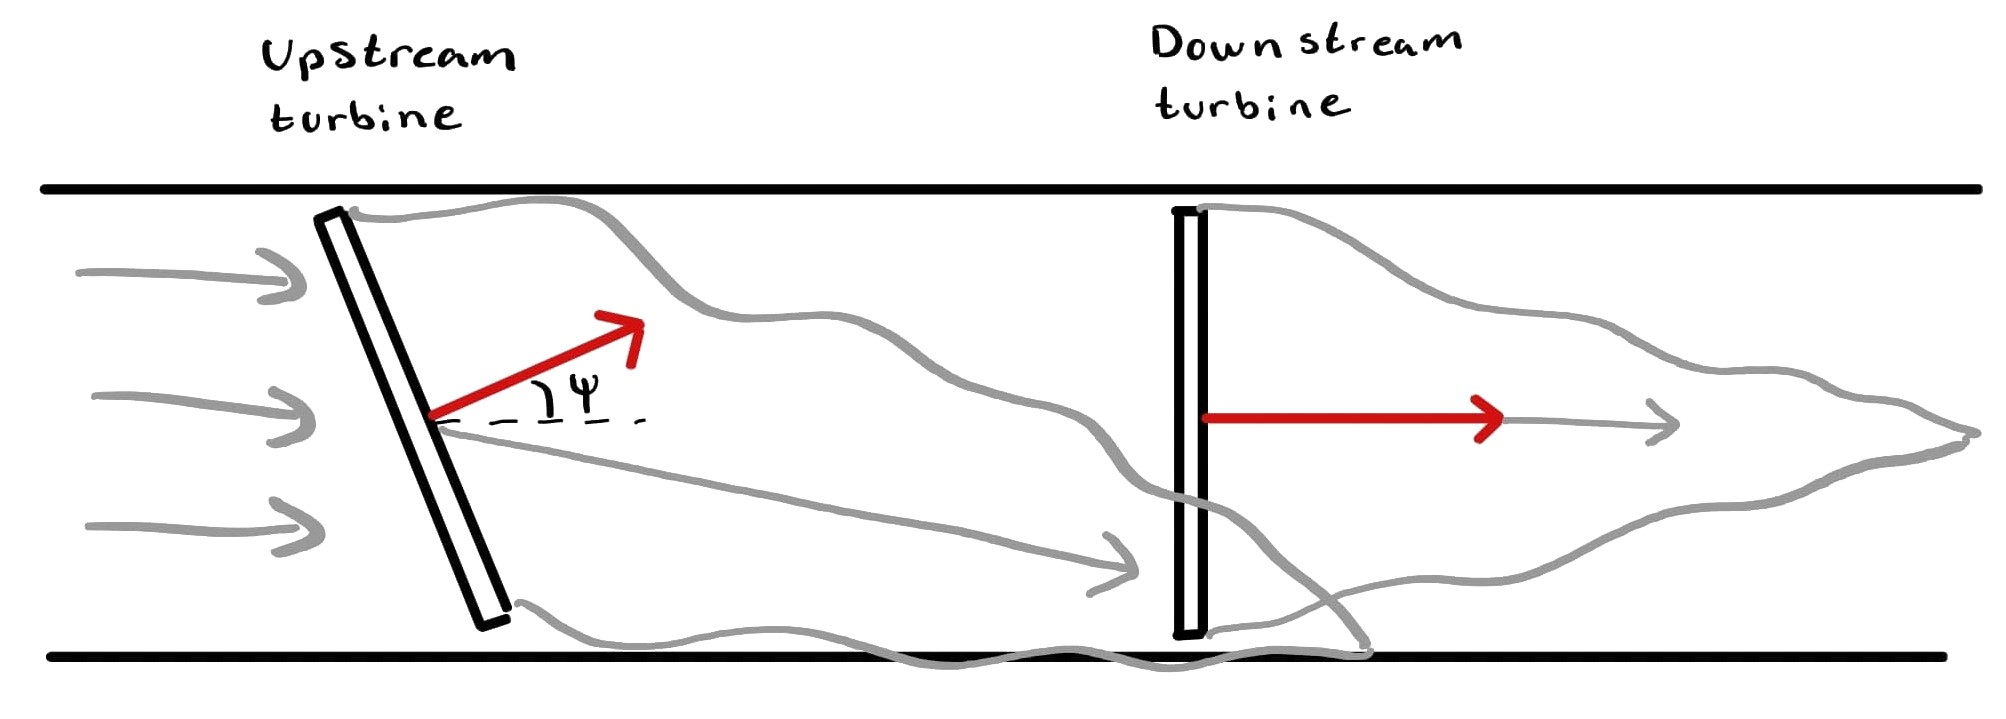
\includegraphics[scale=0.22]{Illustrations/Yaw_illu.jpg}
    \caption{Illustration of yawing on upstream turbine}
    \label{fig:yawingillu}
\end{figure}


For the case of yawing, we can see how the flow creates a thrust perpendicular to the turbine, which in return affects the flow with an equal force in the opposite direction, ultimately resulting in the wake being steered away from the yawing angle. Such measures are generally referred to as Wind farm flow control (WFFC) and will be the primary point of interest throughout this thesis. More specifically, the consequences of turbulent wakes will be examined with a statistical approach through a combination of CFD and aeroelastic calculations. Based on these calculations, the effect of wake steering through yawing will be evaluated, through probabilistic surrogates, to investigate how these results may be used to optimise the total farm on both total power output and relevant loads. The goal is to produce more power without causing unnecessary fatigue and shortening the lifespan. 
